\documentclass{beamer}
\usepackage{graphicx}
\usepackage{subfig}
\usepackage{hyperref}
\usepackage{fancyvrb}
\usepackage[T1]{fontenc} % recommended for languages with accents
\usepackage[utf8]{inputenc}
\usetheme{Darmstadt}

\usepackage[round,authoryear]{natbib}


\title{Topic Detection and Tracking}
\author{
	Marc-André Faucher\\
	Jeff How\\
	Jonathan Villemaire-Krajden
}
\date{June 6, 2013}

\begin{document}

\begin{frame}[plain]
  \titlepage
\end{frame}

\section{Introduction}

\begin{frame}
  \frametitle{Topic Detection and Tracking}
  Wayne (1997) - \textit{automatic techniques for finding topically related materials in streams of data}
\begin{columns}
\begin{column}{.28\textwidth}
  \begin{itemize}
  \item
    \href{http://emm.newsexplorer.eu/NewsExplorer/home/en/latest.html}{EMM NewsExplorer}
  \item
    \href{http://emm.newsbrief.eu/NewsBrief/clusteredition/en/latest.html}{EMM NewsBrief}
  \end{itemize}
\end{column}
\begin{column}{.68\textwidth}
  \begin{figure}[h]
    \centering
    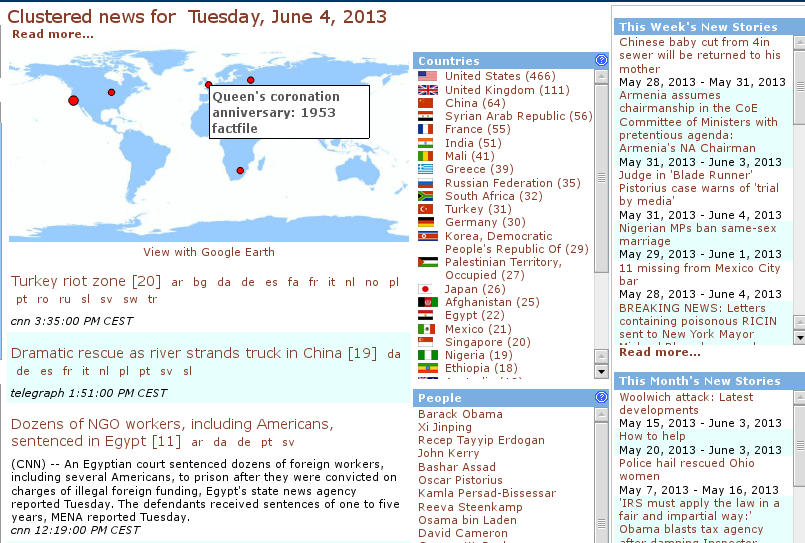
\includegraphics[width=\textwidth]{images/emm_0}
  \end{figure}
\end{column}
\end{columns}
\end{frame}

\begin{frame}
  \frametitle{Terminology}
  \begin{description}
  \item[Story] an article or news broadcast with an underlying focus
  \item[Event] a unique thing that happens at some point in time
  \item[Topic] a set of highly-related events
  \ \\
  \item[Input] a continuous stream of real-time text (stories)
  \item[Output] clusters organized by topic with a leading story
  \end{description}
\end{frame}

\begin{frame}
  \frametitle{Terminology}
  \begin{figure}[h]
    \centering
    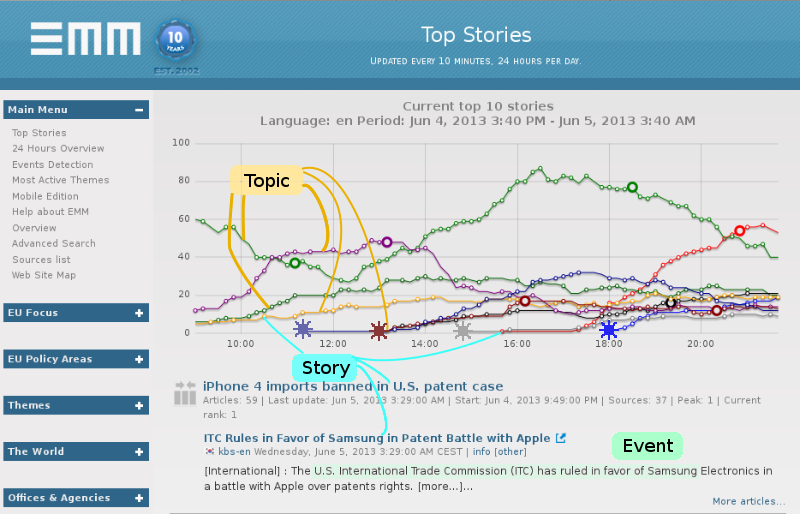
\includegraphics[width=0.9\textwidth]{images/emm_1}
  \end{figure}
\end{frame}

\begin{frame}
	\frametitle{Subtasks}
	\begin{itemize}
		\item Topic Detection
			\begin{itemize}
				\item 1st story
			\end{itemize}
		\item Topic Tracking
			\begin{itemize}
				\item Finding additional stories about a particular topic
				\item Clustering
			\end{itemize}
	\end{itemize}
\end{frame}

\section{Implementation}
\begin{frame}
	\frametitle{Feature Selection}
	\begin{description}
		\item[Lexical] Words, Noun Phrases, Named Entities
		\item[Syntactic] POS tagging (nouns, verbs, proper names)
		\item[Semantic] Temporal language cues (verb tense and temporal NPs)\citep{Makkonen:2003:RATDL}
		\item[Metadata] Timestamps
	\end{description}
\end{frame}

\begin{frame}
	\frametitle{Model Selection}
	Different project used different models to analyze the content.
	\begin{description}
		\item[Vector space] TF-IDF % TODO: ADD CITATIONS
		\item[Probabilistic] Chi-square % TODO: ADD CITATIONS
		\item[Graph-based] Edge counting % TODO: ADD CITATIONS
	\end{description}
\end{frame}
\begin{frame}
	\frametitle{Cluster}
	Stories are grouped through clustering using distance metrics based on the
	model (probabilistic, cosine similarity, etc.):
	\begin{columns}[c]
		\column{3in}
		\begin{itemize}
			\item {\bf K-means:}
				\begin{itemize}
					\item Selecting small \emph{k} with small variance
					\item Centroid represents dominant features
				\end{itemize}
			\item {\bf Hierarchical agglomerative clustering:}
				\begin{itemize}
					\item Provides a hierarchy of clusters 
				\end{itemize}
			\item {\bf KeyGraph link based clustering:}
				\begin{itemize}
					\item Network of features and relations
					\item Topics are identified using network theory
				\end{itemize}
			\item {Advanced Techniques:}
				\begin{itemize}
					\item Latent Dirichlet Allocation (LDA)
					\item Non-negative Matrix Factorization
				\end{itemize}
		\end{itemize}
		\column{1in}
			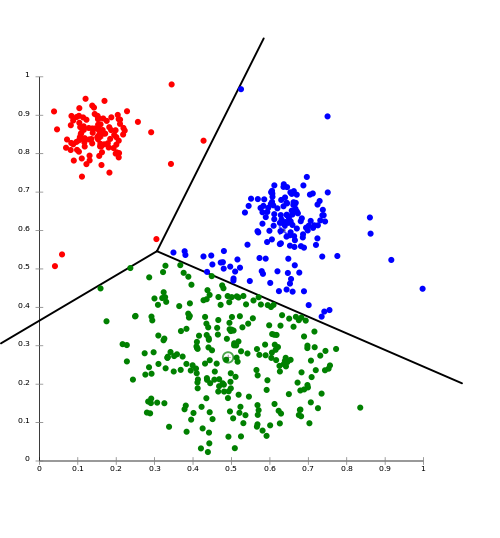
\includegraphics[width=\textwidth]{images/cluster_centroid.png} \\
			\hfill \\
			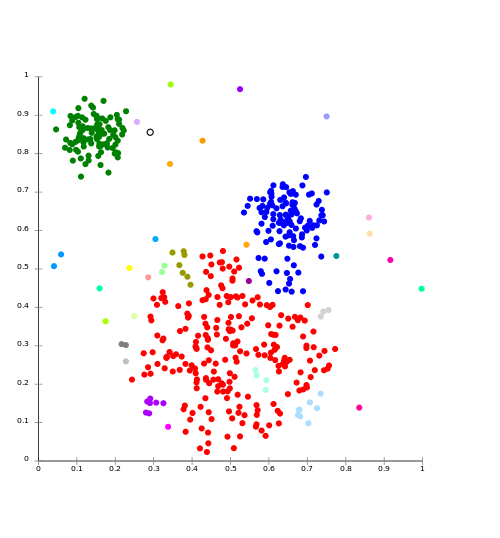
\includegraphics[width=\textwidth]{images/cluster_link.png} \\
	\end{columns}
\end{frame}

\subsection{Examples}
\begin{frame}
	\frametitle{Time-Span \citep{Swan:1999:EST:319950.319956}}
	% TODO: (note to self: this section needs work)
	\begin{itemize}
		\item Entities \& noun phrases with overlapping time-spans constitutes a topic.
		\item Calculate probabilities of time-span overlap for features if independence is assumed.
		\item Merge features, which are statistically dependent ($\chi^2$) in terms of doc occurrence.
	\end{itemize}
	\begin{figure}[h]
		\centering
		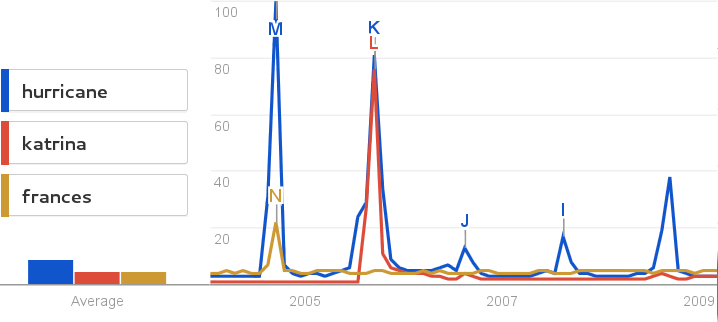
\includegraphics[width=0.5\textwidth]{images/timespan.png}
	\end{figure}
\end{frame}

\subsection{Examples}
\begin{frame}
	\frametitle{Topic Tracking in Tweet Streams \citep{Lin:2011:STA:2020408.2020476}}
	\begin{itemize}
		\item High arrival rate (up to 4000+ tweets per second)
		\item Foreground model: tracks recent topic counts
			\begin{itemize}
				\item History of \emph{h} events
				\item Smoothed with the background model
			\end{itemize}
		\item Background model: long-term estimates of term distributions
			\begin{itemize}
				\item Handles sparsity from limited history of foreground model
			\end{itemize}
		\item Evaluation based off hashtags
	\end{itemize}
\begin{figure}[hb]
\centering
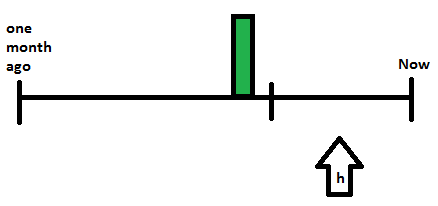
\includegraphics[width=0.5\textwidth]{images/twitter}
\end{figure}
\end{frame}

\section{Conclusion}
\begin{frame}
	\frametitle{Conclusion}
	% TODO: (note to self: this section needs work)
	\begin{itemize}
		\item Topic Detection
		\item Topic Tracking
		\item Implementation: Feature -> Model -> Cluster
		\item Current Application:
			\begin{itemize}
				\item EMM
				\item Google News
			\end{itemize}
	\end{itemize}
\end{frame}

\begin{frame}
  \frametitle{References}
  \footnotesize{
    \bibliographystyle{unsrtnat}
    \bibliography{ref}
  }

\end{frame}

\end{document}


%% \begin{frame}
%% \frametitle{EXAMPLE IMAGE}
%% Some stuff references the image~\ref{fig:example} which can be found bellow.
%% \begin{figure}[h]
%% \centering
%% \includegraphics[width=\textwidth]{opencalais}
%% \caption{An example.}
%% \label{fig:example}
%% \end{figure}
%% \end{frame}
